\documentclass[aps,prx,reprint,superscriptaddress, longbibliography]{revtex4-1}
\usepackage{H1}
\usepackage[pdftex,colorlinks=true]{hyperref}
\hypersetup{citecolor = blue, linktocpage=true}
\usepackage[normalem]{ulem}
\usepackage{color}
\usepackage[usenames,dvipsnames,svgnames,table]{xcolor}
\usepackage{mathtools}
\usepackage{enumerate}

\newcommand{\vedika}[1]{ {\color{red} {{#1}}}}
\newcommand{\david}[1]{ {\color{blue} {{#1}}}}
\newcommand{\charlie}[1]{{\color{Magenta}{{#1}}}}

\newcommand{\Tr}{ \mbox{Tr}}
\renewcommand{\Re}{ \mbox{Re}}
\newcommand{\vb}{v_B}
\newcommand{\I}{\mathbb{I}}
\newcommand{\ip}{i+1}
\newcommand{\mc}[1]{ { \mathcal {{#1}}}}
\newcommand{\Sz}{S_z^{\rm tot}}
\newcommand{\lamv}{\lambda(v)}
\newcommand{\otoc}{{C}({\bf x},t)}
\newcommand{\half}{\frac{1}{2}}
\renewcommand{\ket}[1]{\left|#1\right\rangle}

\begin{document}
\title{Asymmetric butterfly velocities in Hamiltonian and circuit models}
%
\author{Charles Stahl}
\affiliation{\mbox{Department of Physics, Princeton University, Princeton, NJ 08544, USA}}
\affiliation{\mbox{DAMTP}}
\author{Vedika Khemani}
\affiliation{\mbox{Department of Physics, Harvard University, Cambridge, MA 02138, USA}}
\author{David A. Huse}
\affiliation{\mbox{Department of Physics, Princeton University, Princeton, NJ 08544, USA}}

\begin{abstract}
	The butterfly velocity $v_B$ has been proposed as a characteristic velocity for information propagation in local systems. It can be measured by the ballistic spreading of local operators in time (or, equivalently, by out-of-time-ordered commutators). In general, this velocity can depend on the direction of spreading and, indeed, the asymmetry between different directions can be made arbitrarily large using arbitrarily deep quantum circuits. Nevertheless, in all examples of local time-independent Hamiltonians that have been examined thus far, this velocity is independent of the direction of information propagation. In this work, we present two models with asymmetric $v_B$. The first is a time-independent Hamiltonian in one dimension with local, 3-site interactions. The second is a class of local quantum circuits, which we call $n$-staircases, where $n$ serves as a tunable parameter interpolating from $n=1$ with symmetric spreading to $n=\infty$ with completely chiral information progagation.  
\end{abstract}

\maketitle

\section{Introduction}
Understanding the dynamics of isolated quantum systems is a topic of fundamental interest. One central question is how isolated systems undergoing unitary time evolution are able to bring themselves to local thermal equilibrium under their own dynamics. Indeed, while all quantum information is always preserved under unitary evolution, it can get ``scrambled" in highly non-local, experimentally inaccessible degrees of freedom - leading to an effective decoherence that can bring local subsystems to thermal equilibrum. 

A useful window into the scrambling process comes from studying the spreading of initially local perturbations under time evolution. Under Heisenberg evolution, a local operator $O_0$ evolves into $O_0(t) = U^\dagger(t) O_0 U(t)$ with support on a spatial region that grows with time. This spreading of quantum information can be diagnosed by the out-of-time ordered commutator (OTOC) which has recently been studied in a variety of systems ranging from strongly quantum chaotic to integrable. The OTOC is defined as $C(\vec{x},t) = \frac{1}{2} \langle [W_\vec{x}, O_0(t)]^\dagger [W_\vec{x}, O_0]\rangle$, where $W_\vec{x}$, $O_0$ are local norm-one operators near positions $\vec{x}$ and $0$ and the expectation value is taken in an appropriate equilibrium ensemble. If $\vec{x}$ is away from the origin, then $W_\vec{x}$ initially commutes with $O_0$ and the OTOC is zero. As the operator spreads, the OTOC grows to become of order one inside a ``light-cone" bounded in all directions by a propagating front. We focus here on chaotic systems with ballistic information spreading at a ``butterfly speed" $v_B(\hat{\vec{n}})$ which may, in principle, depend on the direction of propagation $\hat{\vec{n}}$. 

Recently, a great deal of insight into the dynamics of operator spreading and quantum entanglement in chaotic systems has been gained by studying various minimally structured coarse-grained models whose time evolution is generated by random unitary circuits. 
Such models are analytically tractable, by design, and are constrained only by locality, unitarity and a few local conservation laws. 
A central assumption, borne out by these studies, is that the time evolution in chaotic systems looks essentially random, so that these ingredients are sufficient for capturing several universal features of the dynamics in thermalizing systems. Several variations have been studied, including unitary circuits that: (i) have random or regular circuit architecture (ii) are random or periodic in time, the latter being so-called Floquet circuits and (iii) have local unitary gates drawn randomly from various ensembles, for example, uniformly from the Haar measure, or randomly from the Clifford group, or uniformly from the Haar measure subject to various local conservation laws. Figure~\ref{fig:circuits} depicts some of these cases. 




Thermalization and operator spreading have recently been important subjects of study. In systems with time-independent Hamiltonians this spreading is often assumed to be symmetric, but there exists no such general constraint. Asymmetric transport is already seen in ``staircase" and ``glider" circuits. The existence of these circuits suggests that some asymmetric Hamiltonians exists, but they might not be general. One goal of this paper is then to describe \charlie{tunable} local asymmetric Hamiltonians.

The case of asymmetric circuits remains interesting. On the edge of a 2-D system, spreading can be chiral even with a finite circuit depth~\cite{PoChiralCircuit}. To be completely chiral with only 1 dimension, however, the circuit will have to be of infinite depth. After identifying the depth of the circuit with its locality \charlie{(how?)} we once again have a trade-off between locality and asymmetry. How asymmetric can a circuit of given depth be?

In this paper we will start by discussing a local Hamiltonian with asymmetric spreading. We show that it is a general Hamiltonian, and provide multiple methods for measuring $v_B$ for left and right spreading. A representative plot can be seen in Fig~\ref{fig:colorplot}. We then discuss staircase circuits in the small- and large-staircase limit and show that in the latter limit the circuit is completely chiral.


\begin{figure}
	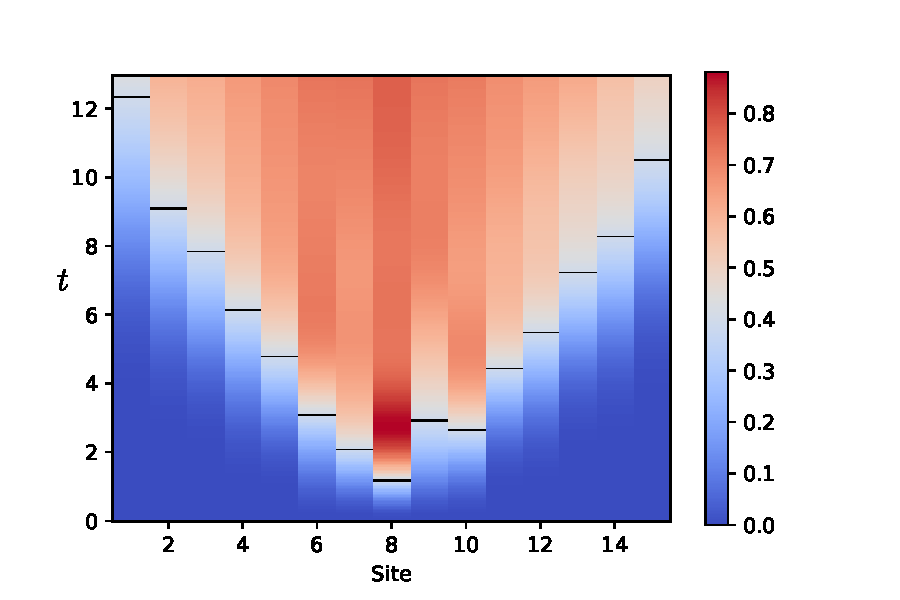
\includegraphics[width=\columnwidth]{colorplot}
	\caption{Evolution of the OTOC for an initially local operator. Data is obtained over 100 disorder samples at $L=15, h=0.35$ with the initial operator at the central site, averaged over 5 disorder realizations. The bars indicate the time at which the OTOC passes 0.4, to emphasize the asymmetry.}
	\label{fig:colorplot}
\end{figure}

%\tableofcontents

\section{Local Hamiltonians}

%In order to define a local Hamiltonian with asymmetric spreading, we have to move away from 2-site interactions because they will have to be symmetric. The space of 3-site Hamiltonians is large ($q^{6} = 64$) so we restrict to SU(2)-symmetric terms. This space is still large \charlie{Does it matter how large?}, but we know we want Hamiltonians that are different in opposite directions. If we restrict further to Hamiltonians antisymmetric under inversion of the spin chain, we are left with only one option, the triple product of spins.

We want a multi-site Hamiltonian in which sites interact only through local interactions. We can accomplish this by defining an $n$-site Hamiltonian for small $n$, and then putting this Hamiltonian on each set of $n$ sites,
\begin{align}
H_{\text{tot}} = \sum_{i=1}^{L-n+1}H_n^{(i)},
\label{eqn:chain}
\end{align}
where $H_n^{(i)}$ is a $n$-site Hamiltonian acting on sites $i$ through $i+n-1$.
$n=2$ will not suffice, because 2-site Hamiltonians are always symmetric with respect to their operator dynamics. To see this, consider the amount of information flowing from site to site. Unitarity preserves the total amount of information so if the 2-site Hamiltonian moves some weight from site $i$ to $i+1$ it must also move an equal amount from site $i+1$ to $i$. 3-site Hamiltonian do not have this constraint, though, and can have asymmetric dynamics.

Instead of looking directly for an asymmetric Hamiltonian, we can find a unitary operator $U(t)$ with the dynamics we want. From that operator we can construct a Hamiltonian that gives $U(t)=e^{-iHt}$. One asymmetric unitary operator is the 3-site cyclic swap $S_{123}$. $S_{123}$ is a unitary operator such that
\begin{align}
S_{123}\ket{\alpha\beta\gamma} =\ket{\gamma\alpha\beta}, \label{eqn:condition}
\end{align}
where $\ket{\alpha\beta\gamma}$ is a product state with state $\ket{\alpha}$ on site 1, etc. The idea of using this operator is that it can transport a state from site 3 to site 1 in 1 step, but takes two applications to move a state from site 1 to site 3.

One way to build the three site swap gate is out of 2-site swap gates $S_{123} = S_{12}S_{23}$. Each 2-site swap interchanges two states, so the action is 
\begin{align}
S_{12}S_{23}\ket{\alpha\beta\gamma} &= S_{12}\ket{\alpha\gamma\beta} = 
\ket{\gamma\alpha\beta}\nonumber\\
&= S_{123}\ket{\alpha\beta\gamma}.
\end{align}
Note that this construction can be extended to $n$ sites to create an $n$-site swap gate. The gate would be a series of overlapping 2-site swap gates. We will come back to this construction to build our asymmetric circuits. The 2-site gates will not be swaps, but the geometry will be the same. \charlie{The problem is that here we apply $S_{12}$ after $S_{23}$ while the staircases seem to be the other way around. I think it might have to do with evolving the state vs the operator.}

It is also possible to build $S_{123}$ out of a time-independent Hamiltonian, so that $U(t)|_{t=1} = e^{-iH_3} = S_{123}$. $H_3$ is the 3-site term we are looking for. There are many ways to construct this Hamiltonian, from directly taking the matrix logarithm to analyzing eigenstates. But the simplest way is to note that exchanging site indices gives $S_{123}^{-1}$ while overall SU(2) rotations leave the gate unchanged. This means $H_3$ should be antisymmetric with respect to site indices and symmetric with respect to SU(2). Therefore $H_3$ is the triple product of the spin at each site.

The Hamiltonian on the full chain is then
\begin{align}
H = \sum_{i=1}^{L-2}{\bf S}_i\cdot({\bf S}_{i+1}\times {\bf S}_{i+2}),\nonumber
\end{align}
The use of 3-site terms has some further consequences. For example, first order perturbation theory will connect site 1 to sites 2 and 3, while second order perturbations connect site 1 to sites 4 and 5. At early time sites 2 will behave the same as site 3, etc., leading to jaggedness in the spreading.
We will correct for this by only looking at odd sites for each analysis. 

\subsection{Degeneracy and Generality}

As is, the model is not general, with one symptom being a large degeneracy at $E=0$. This is an effect of various antisymmetries in the model, which we will call $R_i$, such that $\{H, R_i\}=0$. Each of these operators maps between states of opposite energy, $R_i|E\rangle = |-E\rangle$. Ref.~\cite{IadecolaFSUSY} shows that each $\Tr\;R_i$ provides a lower bound on the $E=0$ degeneracy, which we will call $N_0$. Writing the $E=0$ states as $|\alpha\rangle$,
\begin{align}
\Tr\;R_i = \sum_{\alpha=1}^{N_0}\langle\alpha|R|\alpha\rangle,
\end{align}
But from $R_i^2=1$ we have
\begin{align}
\langle\alpha|R_i|\alpha\rangle=\pm 1.
\end{align}
Thus $\Tr\; R_i < N_0$.

From the design of the model, one such $R_i$ is the inversion operator, $I$. This can be composed with parity operators such as $P_X=\prod_i X_i$ that commute with both $H$ and $I$ to form new $R_i$. Neither operator saturates the degeneracy bound for all $L$, but $\Tr\,I=N_0$ for odd $L$. If we break the SU(2) symmetry to U(1) but leave the inversion symmetry intact then $\Tr\,I$ is exact. If we add a uniform field in the $Z$ direction, then $IP_X$ is an antisymmetry but $I$ is not. In this case $\Tr(IP_X)$ is exact. Taken together, these facts imply that the extra degeneracies for odd $L$ come from interplay between the SU(2) symmetry and inversion antisymmetry.

%From exact diagonalization we know that both $\Tr\;I=N_0$ for even $L$ and $<N_0$ for odd $L$ while $\Tr\;I\,P_X=0$ for even $L$ and $<N_0$ for odd $L$. We can make the exact degeneracy follow the $\Tr\;R_i$ patterns by adding various fields. For example, if we put an inversion-antisymmetric field in the $Z$ direction, tyyyy

We can fully break this degeneracy within each U(1) block by introducing a random field in the $Z$ direction, so the total Hamiltonians is
\begin{align}
H = \sum_{i=1}^{L-2}{\bf S}_i\cdot({\bf S}_{i+1}\times {\bf S}_{i+2}) + 
\sum_{i=1}^{L}h_iS_i^z,
\end{align}
where each $h_i$ has a uniform probability distribution on $[-h,h]$. This field breaks the SU(2) symmetry but leaves the U(1) subgroup intact.

As we continue to increase $h$ the model moves through the thermalizing phase and becomes localized. In the large-$L$ limit the transition from ergodic to localized is a phase transition, described in~\cite{1010.1992v1}. The transition for the present model can be seen in Fig.~\ref{fig:levelrepultrans}, showing the ratio of adjacent energy gaps. Note that at smaller $L$ the model also drifts away from GUE statistics at very small $h$, when the field is no longer large enough to sufficiently lift the $E=0$ degeneracy. In order to avoid both of these regimes, we will perform all calculations with $h=0.35$.

\begin{figure}
	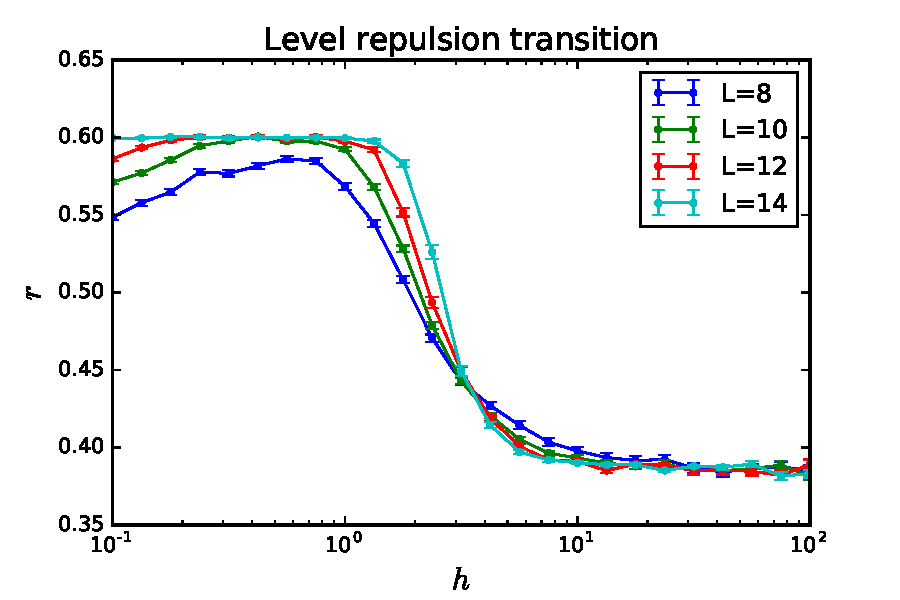
\includegraphics[width=\columnwidth]{levelrepultrans}
	\caption{Phase transition for the model, with level repulsion parameter plotted against field strength. Note that in the thermalizing phase the ratio is $~0.6$ instead of $0.53$ because the statistics are GUE instead of GOE. \charlie{I think I remember Vedika saying this but I can't find where.}}
	\label{fig:levelrepultrans}
\end{figure}

\subsection{Right-weight peaks}

To measure spreading we evolve initially local operators in the Heisenberg picture. For right-spreading the initial operator will be at site 1, and for left-spreading at site $L$.
We will quantify the asymmetry using two metrics. The first is the weight of all operators with right (left) endpoint on site $i$, which we will call the right (left) weight. The other is the OTOC, which will be discussed below.

We use the definition of the right weight from~\cite{KeyserlingkHydro2017}. An arbitrary operator $\cal O$ can be decomposed into Pauli strings ${\cal O} = \sum_\nu c_\nu \sigma^\nu$ where each string contains one of $\{I, X, Y, Z\}$ acting on each site. As the operator evolves in time, so do the $c_\nu$. The right weight is then
\begin{align}
\rho_r(i,t) = \sum_\nu\abs{c_\nu(t)}^2\delta(\text{RHS}(\nu) = i),
\end{align}
where the delta function ensures that we only count Pauli strings that have their right-most non-identity operator on site $i$. The left weight $\rho_l(i,t)$ is defined analogously.  If $\cal O$ is initially local on site $j$ then $\rho_r(i,0) = \rho_l(i,0) = \delta_{ij}$. As the operator spreads, the support of $\rho_r$ moves right at $v_{B,r}$ and $\rho_L$ moves left at $v_{B,l}$. Operator broadening manifests itself in the support of both weights increasing in size. At late times both weights should vanish near $j$.

In the thermalizing phase, the right weights peak as the information front passes. Because of the three-site nature of each term in the Hamiltonian, the right weight and OTOC exhibit an ``odd-even" effect where site 3 peaks before 2, etc. It is possible to account for these by averaging judiciously, or by  looking at only odd sites.  Once this has been done the peaks do travel balistically. At $L=13$, there are enough odd sites that the asymmetry can be seen. 

In order to compare left- and right-weights, we look at  $\rho_r(x_r+1,t)$ and $\rho_l(L-x_l,t)$. This way $x_{r}$ and $x_l$ are distances from the initial operator. Note that $i$ runs from 1 to $L-1$ because it is a label while $x$ runs from 0 to $L$ because it is a distance. This means that $x$ will be even for the sites we are calling odd sites.
Since the peaks broaden at late times, we use the time that $\rho_r(i,t)$ reaches half-maximum to define the location of the peak.
For a picture of the rights weights with their successive peaks, see Fig.~\ref{fig:Rweightpeakshape}.

\begin{figure}
	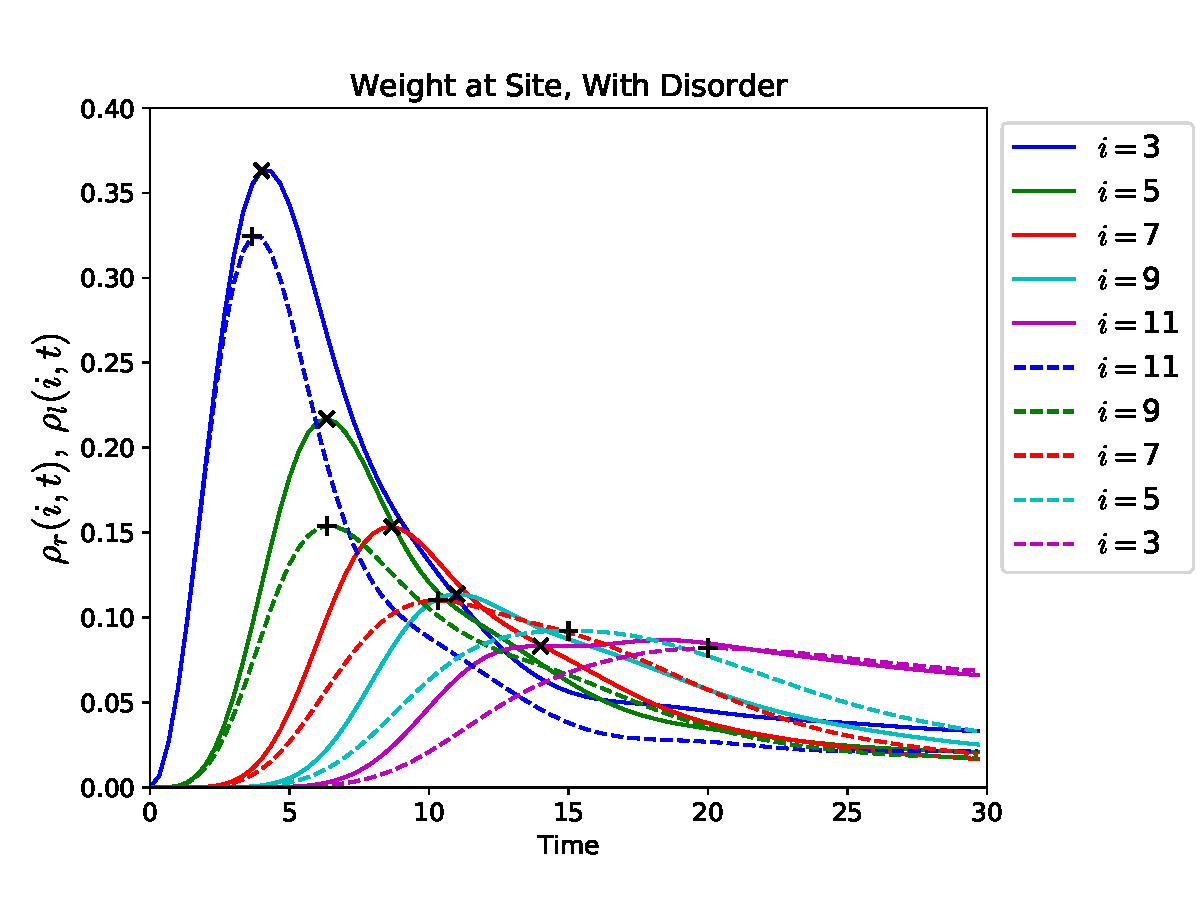
\includegraphics[width=\columnwidth]{Rweightpeakshape}
	\caption{Right weight at odd sites for $L=13$, $h=0.35$, averaged over 100 disorder realizations. For $\rho_r(i,t)$, the initial operator is $Z_1$ while for $\rho_l(i,t)$ the initial operator is $Z_{L}$. The peak travels ballistically. Plots for $x=0$ and $x=L-1=12$ are excluded for clarity. The right-weight is represented by solid lines with a $\times$ where it reaches half peak height, while the left-weight uses dashed lines and a + sign. The right weight peaks earlier at later times, signifying a faster butterfly velocity.
		Later peaks are smaller \charlie{Is this due to broadening?}}
	\label{fig:Rweightpeakshape}
\end{figure}

Fig.~\ref{fig:Rweightpeaktimes} shows the peaks traveling on odd sites. The peaks reach equivalent sites at later times for the left-moving wave, implying $v_{B,l}<v_{B,r}$. We can extract $v_{B,l}$ and $v_{B,r}$ from these curves by fitting linear functions to the peak timings. We find $v_{B,l}=1.011 \pm 0.072$ and $v_{B,r}=0.791 \pm 0.062$. If we instead look at odd sites we find $v_{B,l}=1.106 \pm 0.085$ and $v_{B,r}=0.958 \pm 0.078$. In both cases the difference is larger than the error, although the difference is less exaggerated for odd sites.

\begin{figure}
	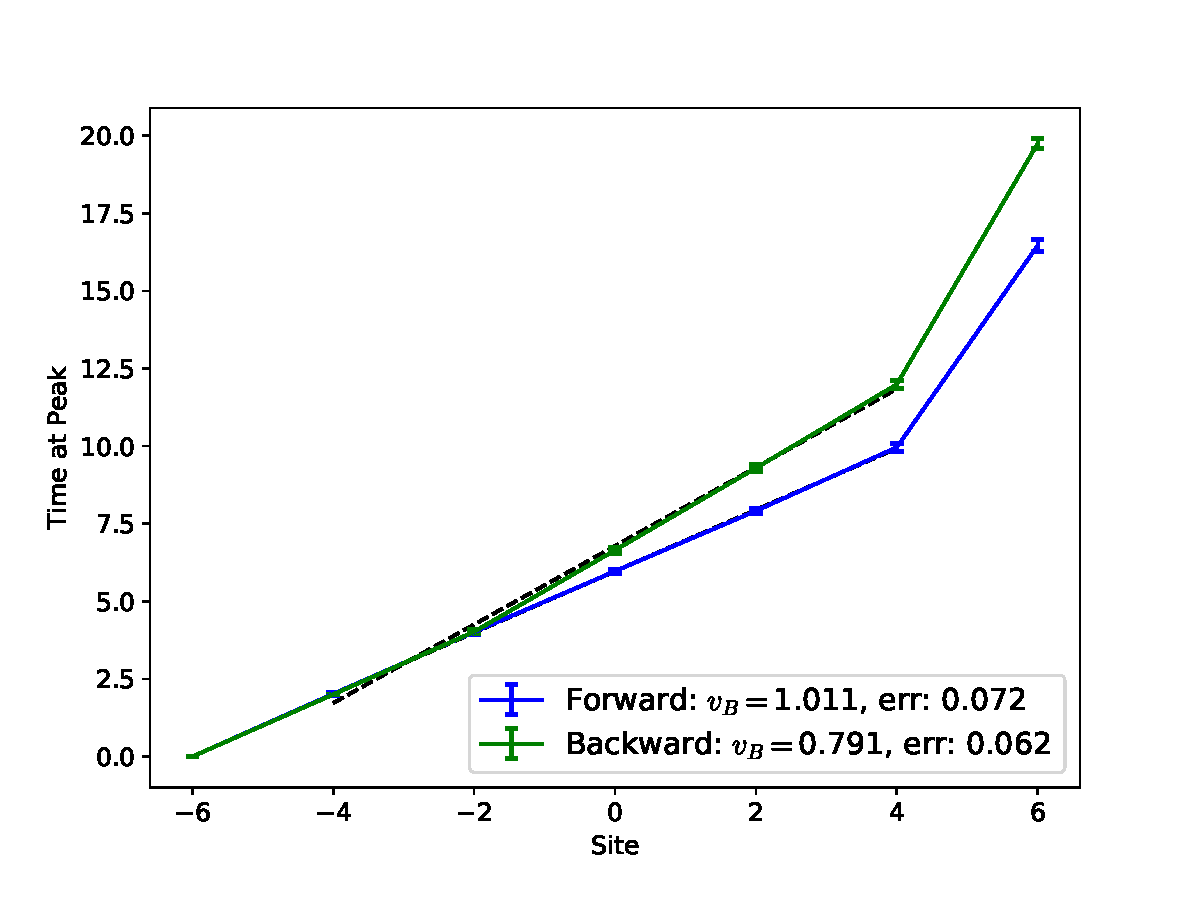
\includegraphics[width=\columnwidth]{Rweighthalftimes}
	\caption{Time of half-peak vs. site. The parameters are the same as in Fig.~\ref{fig:Rweightpeakshape}. Since this is plot of time as a function of distance, the larger slope in the left weight means that $v_B$ is larger for propagation to the right. For the left-weight we plot against $(-\text{site})$ in order to compare left and right.}
	\label{fig:Rweightpeaktimes}
\end{figure}

\subsection{Velocity-dependent Lyapunov exponents}

It is also possible to extract butterfly velocities from the the velocity-dependent Lyapunov exponents, which in turn rely on the OTOC. We define the OTOC as 
\begin{align}
C(i,t) & = \half \langle|[Z_j(t),Z_i(0)]|^2\rangle_{\beta=0}\nonumber\\
&= 1 - \frac{1}{2^{L}}\Re\;\Tr\;[Z_j(t)Z_i(0)Z_j(t)Z_i(0)]
\end{align}
where $j$ is the site of the initial operator and the expectation value in the top row is with respect to a thermal ensemble at infinite temperature. As in the right-weight case, we set $j=1$ to measure $v_{B,r}$ and $j=L-1$ to measure $v_{B,l}$. The OTOC should be order-1 inside the lightcone and exponentially small outside the lightcone defined by $v_B$. Fig.~\ref{fig:colorplot} shows the OTOC for an operator initially local at the center of the chain. The lightcone is approximately where $C(i,t)>.4$, illustrated by the black bars. The lightcone is not monotonic between sites 1 and 2 due to odd-even effects.

\charlie{Move this paragraph to an appendix?}
From conservation of $\Sz$, the Hamiltonian and all relevant operators are block-diagonal, with the size of the $i^\text{th}$ block being $\binom{L}{i}$. For smaller blocks we can compute the trace directly, but for larger blocks this becomes computationally difficult. We then rely on quantum typicality to approximate the trace in the large blocks. For each disorder realization we replace the trace with an average over expectation values in pure states~\cite{Luitz2017}. The pure states are chosen Haar-randomly, and we find that using 5 vectors gives relative errors around 0.05 for blocks larger than $500\times 500$. For smaller blocks we use exact diagonalization.

The VDLEs quantify how fast signals decay along constant-velocity trajectories outside the lightcone. In particular, if the OTOC is measured along the ray defined by each site $i$ at time $t_i = i/v$ for some $v$, then it should decay exponentially,
\begin{align}
C(i, t) \sim e^{\lambda(v)t}\quad\text{for}\quad i = vt.
\end{align}
Ref.~\cite{Khemani2018lambda} gives a thorough exposition and explanation of VDLEs. The name comes from the fact that the Lyapunov exponent defines how fast a signal grows inside a lightcone in a classically chaotic system. 

In the current system, the OTOCs are influenced by the previously-mentioned odd-even effects. We can once again look only at odd sites for sufficiently large $L$ to calculate $\lambda(v)$. Then $v_B$ is the velocity at which $\lambda(v)$ smoothly goes to 0. If we again look at Fig.~\ref{fig:colorplot}, $v_B$ will be the ray that passes through the black bars. Hence, we can already see the asymmetry before calculating $v_B$ explicitly. 

Fig.~\ref{fig:vdle} illustrates the process of finding $\lambda(v)$ and shows the VDLEs for the right-going and left-going OTOCs, estimated from the odd sites. Note that in the top plot the independent variable is distance, so the slope of the best fit line is $\lambda(v)/v$.
Finite-size effects slightly perturb $\lambda(v)$ around $v_B$, but we can see that $v_{B,l} \sim 0.5$ and $v_{B,r} \sim 0.9$. Analysis of the odd sites is less clean, but suggests $v_{B,l} \sim 0.5$ and $v_{B,r} \sim 0.7$.
These are not very close to the velocities estimated from the right weight. Since $v_B$ is \charlie{well defined} only in the thermodynamic limit, we expect these methods to agree as $L\to\infty$.

\begin{figure}
	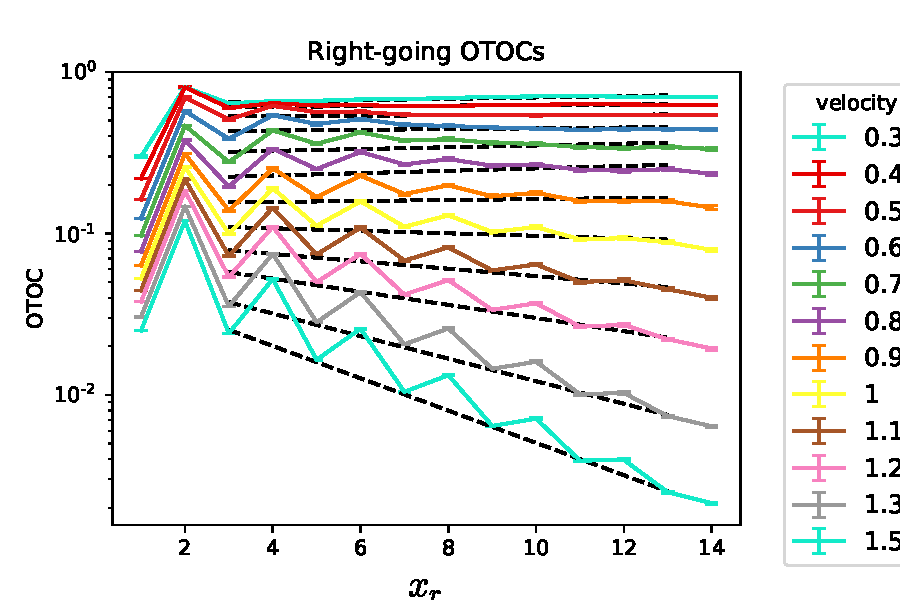
\includegraphics[width=\columnwidth]{oddVDLEfromOTOCs}
	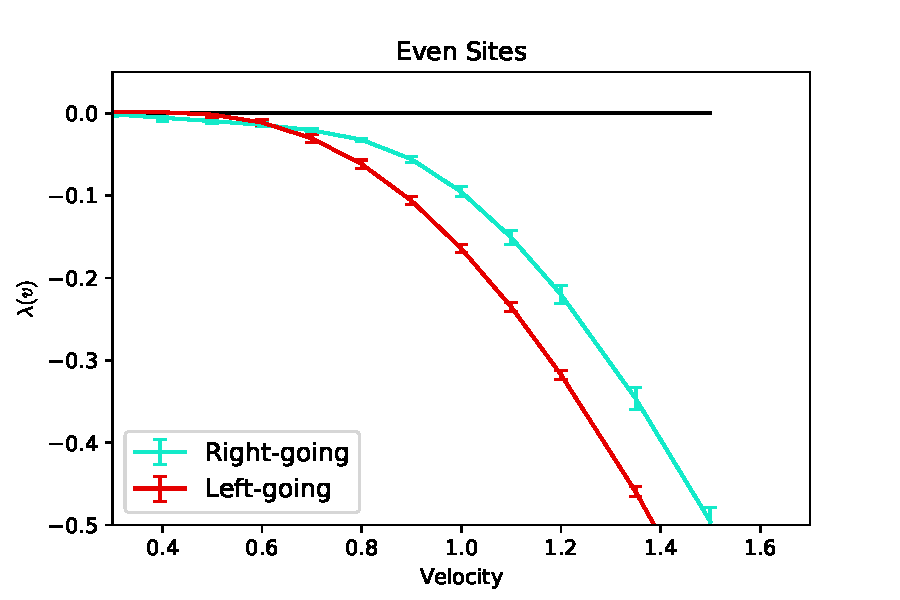
\includegraphics[width=\columnwidth]{oddVDLE}
	\caption{Velocity-dependent Lyapunov exponents extracted from the OTOC on odd sites. The parameters are $L=15, h=0.35$, while the OTOC is as defined in the text with initial operators at sites 1 and $L-1$ respectively. Statistics are obtained from 100 disorder realizations. The top figure shows the early-time right-moving OTOCs on a semilog plot. VDLEs are obtained from the best fit line through odd sites. The lower figure shows $\lambda(v)$. Since $\lambda_r(v)>\lambda_l(v)$, we know $v_{B,r}>v_{B,l}$. \charlie{The data from even sites looks better. I included those figures if you want to switch to that.}}
	\label{fig:vdle}
\end{figure}

\section{Circuit models} \label{sec:circ}

We will now discuss a different system that also displays asymmetric spreading and can be completely chiral in a certain limit. Instead of a time-independent Hamiltonian, this system is a random quantum circuit. Random unitary circuits are discussed in .... The setting for the system is again a spin chain of length $L$, but we allow the dimensionality of each site to be $q$. Eventually we will take the limit $q\to\infty$. At discrete times, unitary operators called gates act on pairs of consecutive sites. We will refer to the spaces between sites as bonds, so that each pair is specified by a bond index. In contrast to the previous section we will refer to the sites with index $i$ and bonds with index $x$. 

Our random circuit will have two sources of randomness. The first will be in the choice of gates, which will be independently chosen from the Haar distribution, which assigns an equal probability to any gate in the space of unitary two-site operators. The second will be in our architecture. A purely random architecture would have a bond chosen at random at each time step. We consider a generalization of this architecture, which we call the staircase architecture, described by the staircase size $n$. The staircase circuit consists of $n$-stairs at random bonds. 
Each $n$-stair is defined by always having strings of $n$ gates act on bonds $x$ through $x+n-1$ in succession. For $n=1$ this is just a random architecture, but large $n$ results in more asymmetric circuits. For $n=L$, the circuit would always have a gate at bond $x+1$ after bond $x$.

We will be interested in circuits with infinite $L$. When $n$ is small we can extract the behavior from systems with finite $L>>n$. For large $n$ we can first take $L\to\infty$ and then $n\to\infty$ or set $n=L$ and take them to $\infty$ together. The behavior does not depend on the order of limits, but for the sake of reasoning about the circuits we will chose the second procedure.

The structure of this section is as follows. Sec.~\ref{sub:entropy} describes how the butterfly velocity for random unitary circuits can be extracted from the entropy growth rate. In Sec.~\ref{sub:classical} we show that the limit $q\to\infty$ results in classical dynamics for the entropy and butterfly velocity. Finally in Sec.~\ref{sub:asym} we explore $v_B$ for these circuits. The transport is symmetric for $n=1$ (random circuit) and completely asymmetric for $n=\infty$. Although the model is not solvable for intermediate $n$, we provide an approximation to the entropy growth function that is correct at $n=1, \infty$.

\subsection{Entropy in random circuits} \label{sub:entropy}

%Before discussing asymmetric circuits we will explain how $v_B$ can be extracted from the growth of entanglement. We will then show that this method is particularly tractable in the large-$q$ limit before applying this method to staircase circuits. 
%Consider a spin chain of $L$ sites, each with dimension $q$. Sites are labeled by $i = 1,\dots, L$ , while the bonds between sites are labeled by $x = 1, \dots, L - 1$. 

Define the entropy function $S(x)$ as the bipartite entanglement entropy across bond $x$. 
After course-graining, the entanglement becomes a continuous function $S(x,t)$. Given a circuit architecture, the entanglement growth rate is to first order only a function of the slope, so we can write \cite{Jonay}
\begin{align}
\frac{\partial S}{\partial t} = \Gamma\left(\frac{\partial S}{\partial x}\right).
\end{align}
It is useful to define the entropy density $s = \partial S / \partial x$, which is so-called because the equilibrium entropy is $S(x, t) = s_\text{eq} \min\{x, L - x\}$.  In the next subsection we will show that the maximal slope is 1. In general the equilibrium slope can be smaller than 1, but since our systems are noisy, $s_\text{eq} = s_\text{max} = 1$.

This function encodes the butterfly velocity as the derivative $\Gamma'(s)|_{s_\text{ext}}$, where $s_\text{ext}$ is one of the extremal entropy densities, 1 or $-1$ in this case. 
\begin{align}
v_{B,l}=\left.\frac{\partial \Gamma}{\partial s}\right|_{s=-1}, 
v_{B,l}=\left.\frac{\partial \Gamma}{\partial s}\right|_{s=-1} 
\label{eqn:vbGamma}
\end{align}
A brief explanation of why this is the case is given in the appendix, while a stronger argument can be found in Ref.~\cite{Jonay}
It follows that any $\Gamma(s)$ with asymmetry at the endpoints will have asymmetric butterfly velocities.

\subsection{Classical dynamics of $q\to\infty$ limit} \label{classical}

We will consider entropy functions $S(x,t)$ defined on a periodic system of length $L$. The boundary conditions are $S(x+L,t) = S(x,t)+sL$, allowing for an overall entanglement density $s$.
Subadditivity tells us ${|S(x + 1)-S(x)|} \le S_1$, where $S_1$ is the entropy at a single site. If we take our logarithms with base $q$, then $S_1 \le 1$.

If a gate acts on bond $x$, it can increase the bipartite entanglement entropy $S(x)$, up to the constraint $|S(x + 1) - S(x)| \le 1$. In the $q\to\infty$ limit, a Haar-randomly chosen gate will, with probability 1, maximally increase the entanglement across the bond it acts on~\cite{nahum2017quantum}. Given the previous constraint, this means that if a gate acts at bond $x$ at time $t$, then $S(x, t+1) = \min\left\lbrace S(x-1,t)+1, S(x+1,t)+1\right\rbrace$. \charlie{Should we explain why?} For the remainder of this paper we will use the $q\to\infty$ limit.

At this point, all quantum effects leave the system, and the dynamics are purely classical. This means it is possible to simulate the circuit without diagonalizing any Hamiltonians or unitary operators. It suffices to consider integer-valued $S(x)$ with $|S(x)-S(x-1)|=1$ for all $x$. A state of this form can be described as a series of up and down steps at each site. If a gate falls on bond $x$, it adds two units of entropy to $S(x)$ iff the step before is down and the step after is up. This classical evolution is deterministic and can be easily simulated.
Since individual circuits have deterministic behavior, we average over circuit architecture (the random placement of $n$-stairs).

Figure \ref{fig:stairs} illustrates the evolution of the entropy function for a 4-stair. The stair consists of 4 individual gates. Each gate has height 2 because if it produces entropy, it produces 2 units. The shaded profile is the initial $S(x)$, while the dashed line shows $S(x)$ after the $n$-stair falls. The first, second, and fourth gates were productive while the third was not.
\begin{figure}
	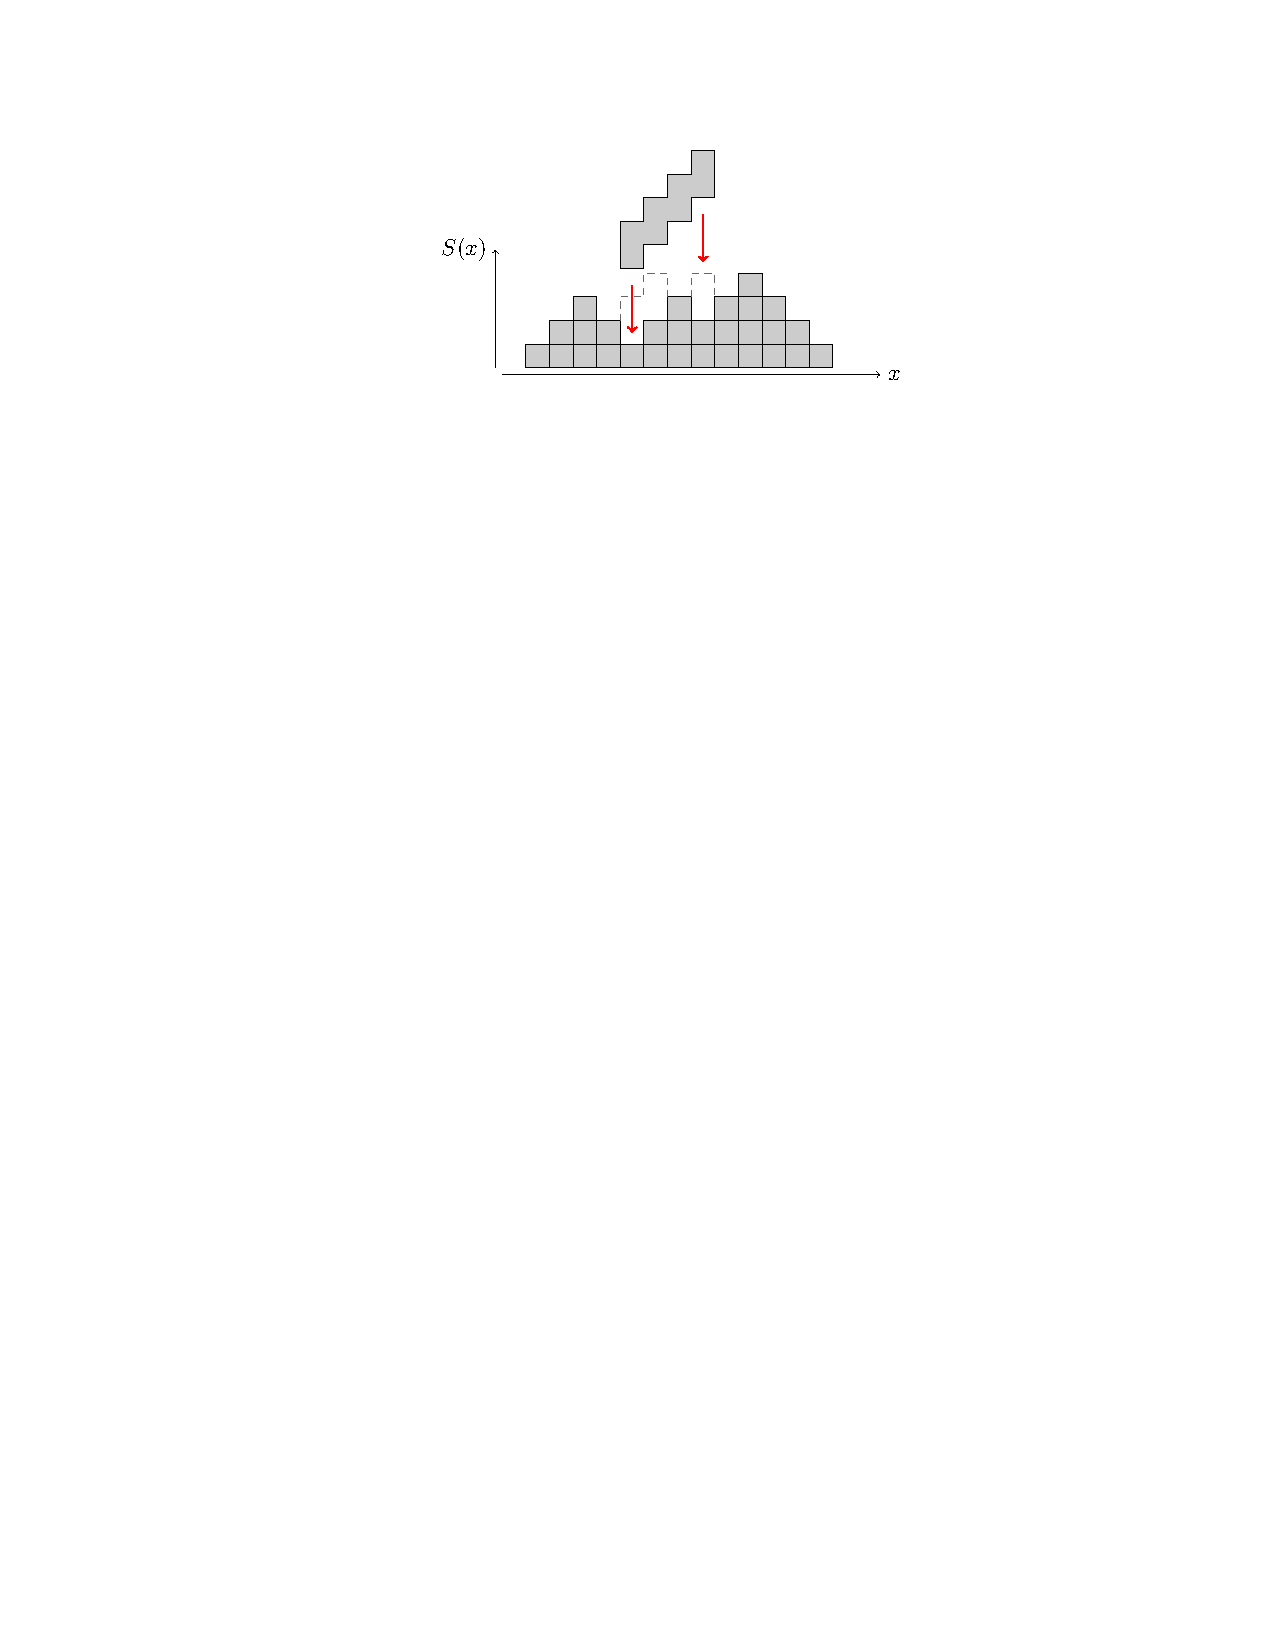
\includegraphics[width=\columnwidth]{stairs}
	\caption{A 4-staircase falling on an example entropy function. Note that each gate raises $S(x)$ by 2 iff $S(x)$ is a local minimum when that gate falls. So the second gates does in fact hit a local minimum because it acts after the first gate.}
	\label{fig:stairs}
\end{figure}
It is already possible to see the origin of the asymmetry. The 4-staircase can only be perfectly effective if it hits the microstate (down, up, up, up, up). Since this microstate has positive slope, it is more likely to be found when the total slope is larger.

The gate rate $\gamma$ is defined as the number of gates per unit time, not staircases.
This means that as if every gate is productive, the entropy growth rate is $\Gamma=2\gamma$.
The rate at which complete staircases fall is $\gamma/n$.

\subsection{Asymmetric $v_B$}

Despite the deterministic evolution of these circuits, they cannot be solved for finite $n>1$. This is due to correlations that arise in the up and down steps of $S(x)$. If these steps were uncorrelated, then a general state could be described solely by the slope $s$. At any bond the probability of an up-step would be $(1+s)/2$ and the probability of down would be $(1-s)/2$. Correlations make the probability of an up dependent on the surrounding steps. 

There are no correlations in the $n=1$ model, so we can exactly solve the entropy growth function.
Since a gate is productive only at a local minimum, the probability that a randomly placed gate is productive is $(1+s)(1-s)/4$. Then the entropy growth rate is the gate rate, times the probability of entropy production, times the entropy produced per gate:
\begin{align}
\Gamma_1(s)=\gamma\frac{(1+s)(1-s)}{4}2 = \gamma\frac{1-s^2}{2}
\end{align}
For larger $n$ we can perform a similar analysis. Although we know correlations will affect the growth rate, hopefully the effect is small. 


2-stairs consist of one gate acting at bond $x$ and one at bond $x+1$. The entropy production of these gates is affected by the slope between the two bonds and the slopes on either side. There are 8 possible configurations of those three slopes, but only 4 result in entropy growth, as shown in table~\ref{tab:2stair}. Weighting each configuration by its probability and the entropy generated, and then multiplying by the staircase rate $\frac{\gamma}{2}$, the growth rate is approximately
\begin{align}
\Gamma_2(s) 
% &= \frac{\gamma}{2} 4\frac{1+s^2}{4}\frac{1+s}{2} + \frac{\gamma}{2}
% 	2\frac{1-ms2}{4}
% 	\left(\frac{1-s}{2} + \frac{1-s}{2} + \frac{1+s}{2}\right) \nonumber\\
&= \frac{\gamma}{2}\frac{1-s^2}{2}\frac{5+s}{2}, \label{eqn:2rate}
\end{align}
We can interpret the factor $\frac{1-s^2}{2}\frac{5+s}{2}$ as the average entropy produced by each staircase. The second factor provides the asymmetry.

\begin{table}
	\centering
	\begin{tabular}{ccc}
		Initial $\to$ Final 
		Configuration        & Probability         & Productivity\\
		$d\,u\,d\to u\,d\,d$ & $\frac{1-s}{2}\frac{1+s}{2}\frac{1-s}{2}$ & 2\\
		$d\,u\,u\to u\,u\,d$ & $\frac{1-s}{2}\frac{1+s}{2}\frac{1+s}{2}$ & 4\\
		$d\,d\,u\to d\,u\,d$ & $\frac{1-s}{2}\frac{1-s}{2}\frac{1+s}{2}$ & 2\\
		$u\,d\,u\to u\,u\,d$ & $\frac{1+s}{2}\frac{1-s}{2}\frac{1+s}{2}$ & 2
	\end{tabular}
	\caption{The four configurations that result in entropy growth for 2-stairs, the relative proportions of the initial states assuming an uncorrelated entropy distribution, and the growth in entropy generated by a 2-stair falling on that configuration. The four configurations that do not result in entropy growth are $u\,u\,u, d\,d\,d, u\,d\,d,$ and $u\,u\,d$.}
	\label{tab:2stair}
\end{table}

We can determine the growth rate for arbitrary length stairs through a recursive relationship. Consider a staircase made of $n$ gates. Like in the $n=2$ case, its growth rate will be proportional to the staircase rate $\frac{\gamma}{n}$ multiplied by the average entanglement generated by each staircase, so we can write
\begin{align}
\Gamma_n(s) = \frac{\gamma}{n}R_n(s), \label{eqn:growthrate}
\end{align}
where $R_n(s)$ is the average entropy production of an $n$-stair. To find an equation for $R_n(s)$, note that the first $n-1$ gates have the same entanglement production as the $(n-1)$-stair. All final states of the $(n-1)$-stair end in a down slope, so the $n$th gate will produce another 2 units of entropy if the last step is up. However, if all $n+1$ initial steps are up no entanglement is generated. 

This behavior is captured by the recursive formula
\begin{align}
R_n(s) = R_{n-1}(s)+2\frac{1+s}{2} - 2\left(\frac{1+s}{2}\right)^{n+1}, \label{eqn:raterecur}
\end{align}
along with the base case $R_0(s)=0$. The solution is
\begin{align}
\Gamma_n(s) = \frac{\gamma}{n}\frac{1+s}{1-s}\bigg(
(1+s)&\left[\left(\frac{1+s}{2}\right)^n-1\right]\nonumber \\
&+n(1-s)\bigg). \label{eqn:growthrate}
\end{align}
Then, from Eqn.~\ref{eqn:vbGamma}, $v_{B,l}=\gamma$ while $v_{B,r}=\half\gamma(n+1)$.
This produces successively more asymmetric butterfly velocities as $n$ increases. 

The question becomes, how much of an effect do the correlations have? 
For small $n$, we can simulate the classical dynamics numerically for finite $L>>n$. This will capture the correct correlation behavior. For the growth rate curves of $n$-stair circuits for $n\le 6$ see Fig.~\ref{fig:compareRates}. 
\begin{figure}
	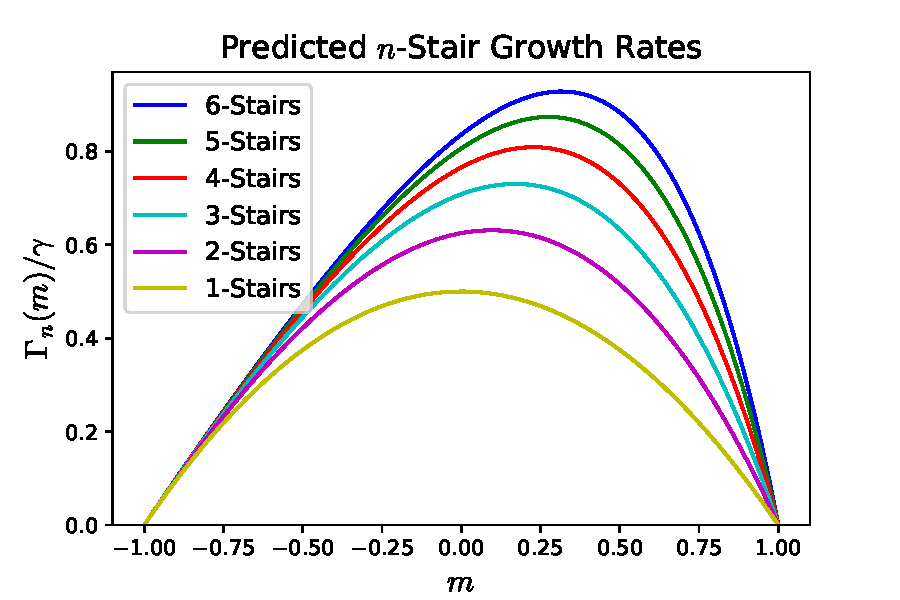
\includegraphics[width=\columnwidth]{predicRates.pdf}
	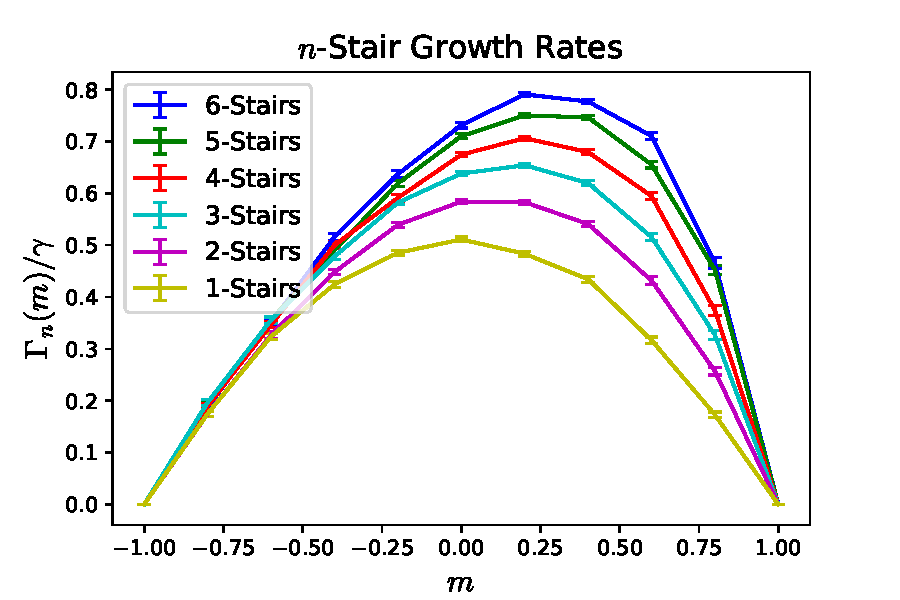
\includegraphics[width=\columnwidth]{compareRates.pdf}
	\caption{Predicted and empirical growth rate as a function of slope for $n$-stair circuits. The predicted growth rate consistently overestimates, but captures the general pattern. The right/forward and left/backward butterfly velocities are the slopes of these curves at their endpoint, indicating that as the left $v_B$ stays constant, the right $v_B$ increases. The appendix includes an argument that the right $v_B$ is unbounded in the large-$n$ limit. All growth rates were calculated using a 100-site spin chain with offset periodic boundary conditions. Rates were calculated from the application of 2,000 gates total, or 20 per site, averaged over the last 80\% of the gates in order to build up correlations, then averaged over 100 trials.}
	\label{fig:compareRates}
\end{figure}
The asymmetry is evident for all $n>1$, and the asymmetry continues to increase as $n$ increases. The growth rates follow the same pattern as the predicted rate, although they are smaller overall. 

Simulation becomes difficult as $n$ increases.
Luckily, as $n$ becomes very large or approaches the size of the system, the correlations again become unimportant. To see this we show that the predicted growth rate is correct at various $s$.
Consider $s = -1, 0,$ and 1 for $n=L$ stairs. At exactly $s=\pm1$ there will be no growth, so we consider an entropy function with a single up or down step before sending $L\to\infty$.

The predicted growth rate is $\Gamma_\infty(s)=\gamma(s+1)$. Near $s=-1$, the entropy profile consists of down steps with a single up step. Then the circuit generates entanglement once every time a staircase falls. We determine $\Gamma_\infty(-1)=\gamma/L$, which approaches 0 as $L$ becomes large.

In the $m = 0$ case, after a gate falls between sites $i$ and $i + 1$, $s_{i+1}$ will be a down slope regardless of whether the gate generated entanglement. Then the next gate falls across sites $i + 1$ and $i+2$. At site $i+2$ $s_{i+2} = u$ with probability $\half$, so on average $\half$ of the gates produce 2 units of entanglement and $\Gamma_\infty(0)=\gamma$. At near-maximal slope nearly all slopes are up, except at the site to the right of the most recent gate. Then the next gate falls at a local minimum with probability 1, and all gates produce 2 units of entanglement, so $\Gamma_\infty(1)=2\gamma$. These growth rates are all consistent with $\Gamma_\infty(s)=\gamma(s+1)$. Using that function, we obtain $v_{B,l}=\gamma$ and $v_{B,r}=\infty$.

Because these rates match the predicated rate, we know it is exact at $s=0, \pm1$. From concavity, the only possible function is then $\Gamma_\infty(s)=\gamma(s+1)$. This shows that our approximation again becomes exact at $n=\infty$ and the system achieves chiral transport. Although we do not know the exact behavior for $1<n<\infty$, we know it interpolates between symmetric and completely asymmetric behavior.

\section{Conclusion}

Asymmetry in $v_B$ is possible, but is limited by locality. In time-independent Hamiltonian systems locality is measured by the range of interactions, while in circuits it is related to the depth. This paper studied both types of systems, showing that local Hamiltonians can support asymmetric spreading and probing spreading in nearly-local circuits. 

The advantages of the Hamiltonian system are that it is a general model. Each site is only a 2-level system. The random field allows the model to be tuned within the thermalizing phase, which could be useful in watching the asymmetry dissipate as the system approaches the phase transition. 

The system studied in this paper is not the only possible 2-nearest-neighbor system. Another interesting direction of research would be how to find maximally asymmetric Hamiltonians for a given interaction length. With more sites per term it would also be possible to study 2-D systems with anisotropic $v_B$.

The class of circuit models studied here provide the opportunity to interpolate between symmetric circuits and completely chiral circuits by varying $n$. One important generalization is to consider finite $q$, the dimension of the Hilbert space at each site. Ref.~\cite{KeyserlingkHydro} suggest that this will lead to a slower $v_B$ as well as $v_E<v_B$. The separate velocity scale $v_E$ leads to operator spreading in individual circuits, not just the ensemble averages this paper discusses.

%We'll want to cite a bunch of people~\cite{Larkinotoc,Lieb72,KitaevSYK,chaosbound,HosurYoshida,ShenkerStanfordButterfly,LocalizedShocks,CotlerRM,RobertsStanford,GuQiStanford,GuQi_rcft,StanfordWeakCoupling,PatelDiffusiveMetal,ChowdhuryON,Galitski_lyapunov,DoraMoessner,LuitzScrambling,ProsenWeakChaos,AleinerOTOC,MotrunichTFIM_otoc,FradkinHuse,ChalkerFloquetChaos,FawziScrambling,opspreadAdam, opspreadCurt, TiborCons, KhemaniCons}.

\section*{Acknowledgements}
We thank many people.

\charlie{Note somewhere about arXiv:1809.02614v1}

\appendix

\section{Butterfly velocity from $\Gamma(s)$}

To see why $\Gamma'(s_\text{ext})$ gives $v_B$, consider a region in which the entropy profile is piecewise linear, with $S'(x<x^*)=s_1$ and $S'(x>x^*)=s_2$. Also note $\Gamma(s)$ is always convex. This is certainly true for the functions considered above, and is also true in general. Then if $s_1<0<s_2$, the transition between the region stays sharp. If it did not, a curve would form with intermediate slopes $s_1<S'(x)<s_2$. But from convexity all of this region would have a faster entanglement growth than $\min\{s_1,s_2\}$ and the peak would reform. Furthermore, this peak location $x^*$ travels at velocity $\dot{x}*=-\frac{\Gamma(s_2)-\Gamma(s_1)}{s_2-s_1}$, the slope of the chord connecting $\Gamma(s_2)$ and $\Gamma(s_1)$.

If instead, $s_2<0<s_1$, the kink does not remain sharp. The sharp point $x^*$ becomes a smooth curve, running tangent to the two linear sections at $x^*_L$ and $x^*_R$. By a similar argument to the above, these features travel at $-\Gamma'(s_{1,2})$. Then the convexity shows that the fastest velocities in the system are $-\Gamma'(s_\text{ext})$. It remains to be shown that $v_B$ cannot be slower than this, but this is just an appendix.

%\bibliography{global}
%\bibliography{}

%\begin{appendix}
%	
%\charlie{Should something go here?}
%
%\end{appendix}

\end{document}
